% Change 'digital' to 'printed' before printing
\documentclass[
  digital, %% This option enables the default options for the
           %% digital version of a document. Replace with `printed`
           %% to enable the default options for the printed version
           %% of a document.
  table,   %% Causes the coloring of tables. Replace with `notable`
           %% to restore plain tables.
  lof,     %% Prints the List of Figures. Replace with `nolof` to
           %% hide the List of Figures.
  lot,     %% Prints the List of Tables. Replace with `nolot` to
           %% hide the List of Tables.
  oneside,
  %% More options are listed in the user guide at
  %% <http://mirrors.ctan.org/macros/latex/contrib/fithesis/guide/mu/fi.pdf>.
]{fithesis3}
%% The following section sets up the locales used in the thesis.
\usepackage[resetfonts]{cmap} %% We need to load the T2A font encoding
\usepackage[main=english, slovak]{babel}

%% For non-Latin scripts, it may be necessary to load additional 
%% fonts:
\usepackage{paratype}
%%1
%% The following section sets up the metadata of the thesis.
\thesissetup{
    date          = 2017/5/22,
    university    = mu,
    faculty       = fi,
    type          = mgr,
    author        = Zuzana Dankovčíková,
    gender        = f,
    advisor       = Bruno Rossi PhD,
    title         = {Custom Roslyn Tool for Static Code Analysis},
    TeXtitle      = {Custom Roslyn Tool for Static Code Analysis},
    keywords      = {roslyn, C\#, compilers, code review, .NET compiler platform, Kentico, analyzer, code fix...},
    TeXkeywords   = {roslyn, C\#, compilers, code review, .NET compiler platform, Kentico, analyzer, code fix..., \ldots},
}
\thesislong{abstract}{
    TODO: This is the abstract ...
}
\thesislong{thanks}{
    TODO: This is the acknowledgement\dots

}

%% The following section sets up the bibliography.
\usepackage{csquotes}
\usepackage[              %% When typesetting the bibliography, the
  backend=biber,          %% `numeric` style will be used for the
  style=numeric,          %% entries and the `numeric-comp` style
  citestyle=numeric-comp, %% for the references to the entries. The
  sorting=none,           %% entries will be sorted in cite order.
  sortlocale=auto         %% For more unformation about the available
]{biblatex}               %% `style`s and `citestyles`, see:
%% <http://mirrors.ctan.org/macros/latex/contrib/biblatex/doc/biblatex.pdf>.
\addbibresource{mybib.bib} %% The bibliograpic database within
                          %% the file `example.bib` will be used.

\usepackage{makeidx}      %% The `makeidx` package contains
\makeindex                %% helper commands for index typesetting.

%% These additional packages are used within the document:
\usepackage{paralist}
\usepackage{amsmath}
\usepackage{amsthm}
\usepackage{amsfonts}
\usepackage{url}
\usepackage{menukeys}
\usepackage{tikz-qtree}

\begin{document}
% =================================================================
% ============================= CHAPTER 1 =========================
% =================================================================
  \chapter{Introduction}
TODO...
%Ideas:
%
%What is code quality, why is it important, tool that support it.. compilers, diversion ... aaaand here comes Roslyn which provides compiler as a platform.  
%
%In~the~.NET world, the~compiler used~to~be a~black box that given the~file paths to~the~source text, produced an~executable. In~order~to do that, compiler has to collect large amount of~information about the~code it is processing. This knowledge, however, was unavailable to~anyone but the~compiler itself and it was immediately forgotten once the~translated output was produced~\cite{roslyn-overview-github}. 
%
%Why is this an~issue when for decades this black-boxes served us well? Programmers are increasingly becoming reliant~upon the~powerful integrated development environments (IDEs). Features like IntelliSense, intelligent rename, refactoring or~"Find all references" are key~to~developers' productivity; and~even more so in~an~enterprise-size systems. 
%
%This gave a~rise to~number of~tools that analyze the~code for common issues and are able to~suggest a~refactoring. The problem is that that such~tool needs to~parse the~code first in~order~to be~able~to~understand and~analyze it. As a result companies need to invest fair amount of resources to duplicate the logic that the .NET compiler already possesses. Not only is it possible that the compiler and the tool may disagree on some specific piece of code, but with every new version of C\# the tool needs to be updated to handle new language features\cite{dot-net-development-using-the-compiler-api}.
%
%With roslyn.. etc. etc. .. API for analysis.. use in companies for custom analyzers... etc. etc....
% https://github.com/dotnet/roslyn/wiki/Roslyn Overview -- motivation
%Make sure to stress out that ".NET Compiler Platform" and "Roslyn" names will be used interchangably as it is in Roslyn Succinctly on page 11.

% =================================================================
% ============================= CHAPTER 2 =========================
% =================================================================
\chapter{Compilers}
\label{chap:compilers}
As~per~\cite{dragon-book}, a compiler is a~program that can read a~program in a~\textit{source} language and~translate it into a~semantically equivalent program in~a~\textit{target} language while reporting any errors detected in~the~translation process. The compiler may sometimes rely on other programs. For example, \textit{preprocessor} is responsible for collecting the source code to be fed to the compiler by expanding shorthands (macros) into source language statements. 

The compilation process can be divided into two parts: \textit{analysis} and \textit{synthesis}; commonly referred to as \textit{front end} and \textit{back end} of the compiler.

The purpose of the analysis part is to break up the source program into chunks and build up a grammatical structure that it corresponds to, based on the source language grammar. This structure is subsequently transformed into an intermediate representation of the source program. Along the way, the compiler collects information about the program and stores it into a data structure called \textit{symbol table}. If any errors in syntax or semantics are encountered, analysis part shall inform the programmer about the problem. Otherwise, both intermediate representation and symbol table are passed to the synthesis part where they are used for the construction of the target program.

The two main steps of compilation process internally consist of different phases as shown in Figure~\ref{fig:compiler-phases}. Each phase transforms one representation of source language into another, and passes it to the following phase while working with the symbol table during the process. In synthesis phase, an optional machine-independent optimizations can take place and are done on the top of intermediate representation. After target machine code is generated, additional machine-dependent code optimizations are performed.

\begin{figure}[h!]
		\centering
			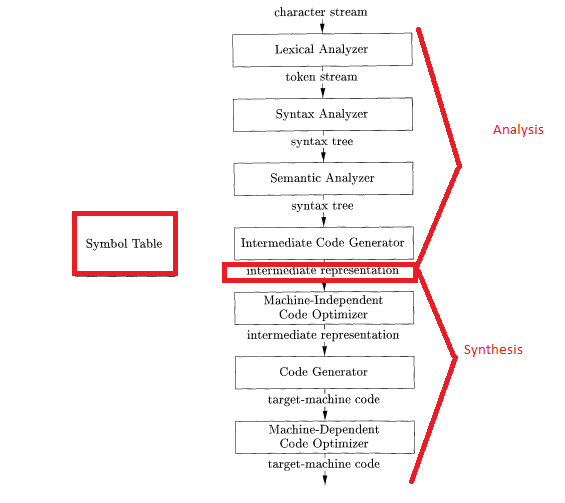
\includegraphics[scale=0.75]{img/compiler-phases}
		\caption{TODO: Phases of the compiler~\cite{dragon-book}}
		\label{fig:compiler-phases}
\end{figure}

For the purpose of this thesis, mainly the analysis part is relevant and following section will elaborate on its respective phases.

  \section{Lexical analysis}
The compilation process starts with \textit{lexical analysis} or \textit{scanning}. The scanner transforms stream of characters of the source program, as written by the programmer, into the series of meaningful sequences called \textit{lexemes}. Most programming languages allow for an arbitrary number of white spaces to be present in the source text to aid readability. However, white spaces, similarly as comments, are unimportant for the target code generation itself, and thus the lexical analyzer is responsible for discarding them completely.

In order to be able to correctly recognize the lexeme, lexical analyzer may need to read ahead. For example, in C--like languages if the scanner sees \texttt{<} character, it cannot decide whether it is a lexeme for \textit{"less than"} operator or it is s part of \textit{"less then or equal to"} lexeme. In order to do that, it needs to read ahead and see if the following character is \texttt{=} or not. Reading ahead is usually implemented with an input buffer which the lexical analyzer can read from and push back to. The use of buffer also boosts the performance as fetching block of characters is more efficient as fetching one at a time~\cite{dragon-book}.

The lexical analyzer typically uses regular expressions to identify the lexemes and for each lexeme, it outputs a \textit{token} (or \textit{token object}) of the form 
\begin{equation}
  \langle token \textnormal{-} name, attribute \textnormal{-} name \rangle \textnormal{.}
\end{equation}

\noindent
For an input sequence 
\begin{equation}
  total = 42 + base * interest
\end{equation}
 
the scanner output could be
\begin{equation}
  \langle id, 0 \rangle 
  \langle = \rangle 
  \langle num, 1 \rangle 
  \langle + \rangle 
  \langle id, 2 \rangle 
  \langle * \rangle 
  \langle id, 3 \rangle
\end{equation}

Lexemes can be divided into logical groups such as identifiers, relational operators, arithmetical operators, constants or keywords as seen in the example above. The scanner often uses regular expressions to identify tokens.

Each identifier (\texttt{id}) has an attribute which points to the entry of the symbol table, where information about identifier name, type or position in the source text is stored. Similar holds for constants like "42" in the example. In the (2.3) example, the assignment and addition symbols do not have attributes but different representation can be used, such as $ \langle bin \textnormal{-} op, 2 \rangle $. In this case, \texttt{bin-op} would denote it is a binary operator and number two would be a pointer to symbol table with all symbols for binary operations while the second index suggests that it represents an addition.

  \section{Syntax Analysis}
The stream of token objects along with partially populated symbol table is an input for the subsequent compiler phase -- \textit{syntax analysis} or \textit{parsing}. The parser has to verify that the sequence of token names can be produced by the grammar for the source language and for a well-formed program, it shall output a \textit{syntax tree} or often referred to as an abstract syntax tree (AST)\footnote{The AST is an intermediate representation of source program in which each interior node represents an operation (programming construct) with the children of the node representing the arguments of that operation. As opposed to \textit{parse syntax tree}, in which interior nodes are nonterminals of the grammar, ASTs are more lightweight and they might omit some nodes which exist purely as a result of grammar's production rules~\cite{secure-programming-with-sca}.}.

The resulting AST for the token stream generated in (2.2) is depicted in Figure~\ref{fig:compilers-abstract-syntax-tree}. The tree shows how multiplication precedence rule of the language's grammar was applied on the expression.

\begin{figure}
  \centering
  \begin{tikzpicture}
  \tikzset{every tree node/.style={align=center,anchor=north}}
  \Tree[.{$\langle = \rangle$} 
        [.{$\langle id, 0 \rangle$} ]
        [.{$\langle + \rangle$} 
          [.{$\langle num, 1 \rangle $} ]
          [.{$\langle * \rangle $} 
            [.{$\langle id, 2 \rangle $} ]
            [.{$\langle id, 3 \rangle $} ]
          ]
        ]
      ]
  \end{tikzpicture}
  \caption{Abstract Syntax Tree}
  \label{fig:compilers-abstract-syntax-tree}
\end{figure}

The syntax analyzer uses a context free grammar (CFG) to form the syntax tree. The CFG is defined by a 4-tuple consisting of:
\begin{description}
  \item[Terminals] -- token names (first component of the token) as obtained from the previous compilation step.
  \item[Nonterminals] -- syntactic variables that help to impose the hierarchical structure of the language and represent set of strings.
  \item[Start symbol] -- a special nonterminal which set of strings represents the language generated by the grammar.
  \item[Productions] -- rules that specify how nonterminals can be rewritten to sequences of zero or more terminal and nonterminal symbols. 
\end{description}

An example of a production denoting the construction of a \texttt{while-cycle} would be
\begin{equation}
  stmt 
  \rightarrow 
  \textbf{while}\ 
  \textbf{(}\ expr\ \textbf{)}\ 
  \textbf{\{}\ stmt\ \textbf{\}} 
  \textnormal{,}
\end{equation}
\noindent
where nonterminals \textit{stmt} and \textit{expr} stand for a statement and expression respectively (defined further by other productions). Symbols in bold represent terminals of the grammar -- open and close parenthesis, and curly braces, \texttt{while} keyword.

  \subsection{Error Handling}
  % TODO bullet points
There are several types of errors that can be encountered during the compilation process:
\begin{compactitem}
  \item\textbf{lexical errors} such as misspelling the identifier name,
  \item\textbf{syntactic errors} like missing semicolon,
  \item\textbf{semantic error} for example incorrect number of function arguments,
  \item\textbf{logical errors} that do not really prevent the program from compiling but can indicate possible mistakes (for instance using the assignment operator \texttt{=} instead of the comparison operator \texttt{==} in condition of an if-statement).
\end{compactitem} 
%\textit{Lexical errors} such as misspelling the identifier name, \textit{syntactic errors} like missing semicolon, \textit{semantic error}, for example incorrect number of function arguments or \textit{logical errors} that do not really prevent the program from compiling but can indicate possible mistakes (for instance using the assignment operator \texttt{=} instead of the comparison operator \texttt{==} in condition of an if-statement).

It's parser responsibility to report the presence of potential syntactic error and recover from the error in order to continue with syntactic analysis and be able to detect any subsequent errors. There are two main strategies for the error recovery~\cite{dragon-book}

  \subsubsection{Panic-Mode Recovery}
In this method, after parser encounters an error, it searches for a \textit{synchronizing token} (usually delimiters such as semicolon or close brace) and until found, all the symbols are thrown away one by one. Even though panic-mode recovery often discards significant amount of input while searching for the synchronization token, it is guaranteed not to end up in an infinite loop.

  \subsubsection{Phrase-Level Recovery}
Another approach the parser can take to recover from an erroneous input is to try to perform a local correction. This can be achieved by replacing the prefix of the following input by some tokens that would enable syntactic analyzer to continue parsing. A prime example of phrase-level recovery is inserting a missing semicolon or replacing comma with a semicolon. Even though this technique is very powerful, as it can cope with all possible problems in the input, it might lead to infinite loops (e.g. always inserting symbols ahead of the current symbol).

  \section{Semantic Analysis}
While syntax analysis is able to check the conformance of the program to the grammar of the source language, it is not an ultimate tool. Some language rules cannot be implied by CFG and an additional step is needed to ensure semantic consistency. To do this, the semantic analyzer uses the AST and the information from symbol tables collected in previous phases. While working, it can also add more details about symbols or even modify the AST. 

A vital part of semantic analysis for any statically typed language\footnote{In statically typed language, type errors are reported by compiler during translation process, whereas in dynamically typed programming languages conversions between incompatible types are only discovered during runtime and can cause program failure.} is \textit{type checking}. Semantic analyzer has to ensure, that each operator is applied to matching operands. For example, a multiplication operator can be called with either a pair of integers or a pair of floating-point numbers, that also implies the result of the operation. If the semantic analyzer encounters an expression where multiplication is used with numbers of different types, it must perform a type conversion called \textit{coercion}. To coerce the integer into floating-point representation it may be necessary to alter the AST and insert an additional node to explicitly state that integer should be treated as floating-point~\cite{dragon-book}. 

Semantic analyzer utilizes the information from symbol table to perform all sorts of other checks, to prevent semantic errors such as:
\begin{compactitem}
  \item \textbf{wrong arguments} -- number and types of arguments applied to a function call,
  \item \textbf{multiple declaration} -- variable with the same name declared more than once in one scope,
  \item \textbf{undeclared variable} -- usage of a variable before its declaration.
\end{compactitem}
    
  \section{Intermediate Code Generation}
The semantic analysis is followed by the \textit{intermediate code generation} which completes the front end part of the compilation process. Depending on the specific compiler implementation, the \textit{intermediate representation} (\textit{IR}) that is the result of this phase can take different forms. The IR should be easy to produce and easy to translate into the target machine code. For some compilers, the IR may be the abstract syntax tree itself.

\bigskip
Together with symbol table, IR is passed to back end part of compiler -- synthesis, where machine independent optimizations can be performed. These contain \textit{control flow analysis} where control flow graph is constructed and utilized in subsequent \textit{data flow analysis}. As a result of these optimizations, compiler might remove dead code from the IR or perform other optimizations that will lead to shorter and more efficient target code.

\bigskip
The following chapters on static code analysis and .NET compiler platform will build upon fundamentals presented here and show how these concepts are relevant when considering the implementation of a static code analyzer.

% =================================================================
% ============================= CHAPTER 3 =========================
% =================================================================
  \newpage
\chapter{Static Code Analysis}
\label{chap:static-code-analysis}
Static code analysis refers to a process of assessing the program based on its form, structure, content and documentation and reasoning over its possible behaviours without actually executing the code. The aim of static analysis is to check the compliance to specific rules and identify parts of the program that might lead to possible vulnerabilities. The term static code analysis is mostly used when speaking of an automated tool. In contrast, \textit{code inspections} or \textit{code reviews} are performed by humans and can benefit from using static code analysis tools~\cite{oswap-sca, ppt-sca}.

% \section{Why}
% Describe why not only testig, differences, what is code quality
%Software quality is~\cite{software-engineering-practicioners-approach}: \textit{"An effective software process applied in a manner that creates a useful product that provides measurable value for those who produce it and those who use it."} This definition can be viewed from two perspectives:
%\begin{compactitem}
%  \item \textbf{user (customer) perspective} -- \textit{a useful product}
%  \item \textbf{developer perspective} -- \textit{an effective software process}
%\end{compactitem}
%
%Software quality is represented by internal and external software characteristics~\cite{code-complete}.
%
%External quality characteristics are ones that the user of the software product is primarily concerned with. These are for example correctness, usability, efficiency, reliability, integrity, adaptability, accuracy and robustness. 
%
%On the other hand, internal characteristics such as maintainability, flexibility, portability, reusability, readability and testability; are only important for programmers and have no visible customer value. 
%
%However, these attributes influence the external characteristics. For example, if software is not readable internally, it is hard to find and fix bugs which directly affect users perception of software's reliability and correctness. For a software company, high internal quality means less maintenance effort, faster time-to-market, fewer bug and thus reduced customer support. It enables engineers to focus on developing new features rather then dealing with unmaintainable code base. 
%  
%While external quality, or conformance to customer requirements, is mostly -?- checked -?- by functional testing, there is more to software quality. Next sections will take a look at who overall quality of code can be raised... OMG this is such a wierd paragraph... 
%
%\section{...}
%  
%\section{Code review process}
%- Code review process = manual inspections of the code
%- types of code review: pair programming, formal, informal
%-where does the SCA fit here
%
%"A static analysis
%tool can make the code review process faster and more fruitful by hypothesizing
%a set of potential problems for consideration during a code review." [secure-programming p.13]
%
%Pridat obrzok z SQ lecture 10 slide 48 a premostit tak ku SCA "The Review Cycle" Secure programming p 48
%
%\subsection{How does it fit to SDLC}
%- integration to IDE, 
%- SCA part of code review process
%- is cheaper when it finds bug than testing

\section{Source Code vs. Compiled Code Analysis}
There are two different approaches when analyzing a program by an automated tool: analyzing the source code (as seen by the compiler), and analyzing the compiled code -- either some form of byte code~\footnote{An intermediate representation of a program, also known as "portable code", which is often for just-in-time compilation by interpreters.} or an executable.

Sometimes it might be very complicated, or even infeasible, to obtain the actual source code of the program to be analyzed and the only possibility is to analyze the executable code. When the tool is looking at a compiled version of the program, the ambiguity of how the source will be translated by the compiler is removed and thus the analyzer does not need to guess. 

However, analyzing compiled code can be very complex. Even if the tool manages to decode the binary, it lacks the original type information. Moreover, the optimizations performed by the compiler obscure the original meaning of the program and making sense of semantics out of implementation may be unattainable. Likewise, if the error is found, reporting it to the programmer can be challenging since there is not always a clear mapping from binary back to source. 

Although the above-mentioned complications speak clearly against analyzing binaries, the situation is different when analyzing byte code formats (such as Java bytecode), where the type and debugging information is present. The following sections will discuss the theory behind the static code analysis.

\section{How It Works}
There are many tools for static code analysis and each can analyze different flaws in the program. However, for a majority of them, the basic structure looks the same, as depicted in Figure~\ref{fig:static-code-analysis-internals}.

\begin{figure}[h!]
		\centering
			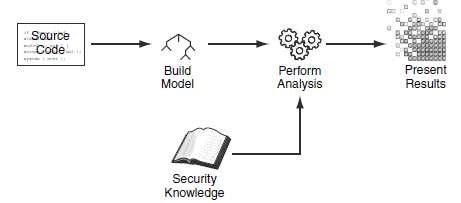
\includegraphics[scale=0.75]{img/static-code-analysis-internals}
		\caption{The process of static analysis~\cite{secure-programming-sca}}
		\label{fig:static-code-analysis-internals}
\end{figure}


\subsection{Build a Model}
In order to analyze the program, the analysis tool must first understand it. Therefore, the initial task is to \textit{create a structured model} that represents the source code. This model has a lot in common with the AST and symbol tables that were discussed in Chapter~\ref{chap:compilers}. In fact, model building phase of static code analyzers closely mimics the front end part of the compilation process, executing lexical analysis, parsing and semantic analysis.

\subsection{Perform the analysis}
After obtaining the model, the next step is to perform the actual analysis. Many different algorithms can be applied in this step and it is common that they are combined into one solution. The approaches are often derived from techniques used by the compilers, specifically:

\subsubsection{Control Flow}
In order to explore different execution paths that can take place when the program is executed, the static code analysis tool can construct a \textit{control flow graph} on the top of the AST. The nodes of the graph represent basic blocks -- sequences of program instructions that will be all executed once block is entered. The edges between basic blocks represent different paths that the program can take depending on matched conditions. Any back edges in the graph signal potential loops in the program execution.

\subsubsection{Tracking Data Flow}
Data flow analysis is used to examine how data passes through the program. Compilers utilize data flow analysis when doing code optimizations in order to remove unreachable code and allocate registers. An example of how data flow analysis can be used by static analysis tools is to check that memory is always freed only once -- function \texttt{free(p)} was called at most once with the address stored in pointer \texttt{p}.

\subsubsection{Taint Analysis}
According to~\cite{oswap-sca}, taint analysis attempts to identify variables containing possibly tainted user input using data flow analysis technique. If these variables are used as arguments to vulnerable functions without being sanitized first, the tool reports their usage as vulnerable. The taint propagation analysis is particularly relevant for security analysis, a prime example being the detection of a potential SQL injection.

\subsection{Rules}
As stated in~\cite{sca-for-security}: \textit{"...if a rule hasn’t been written yet to find a particular problem, the tool will never find that problem."} This implies that the rules that specify what the static analysis tool should report are just as important (or even more important) as the heuristics and algorithms implemented by the tool. Best tools for static code analysis externalize the rule set in order to easily add, remove or alter the rules, without modifying the tool itself.

\subsection{Report the results}
An often overlooked part of the static analysis is the result reporting. The~\cite{coverity-sca} asserts, that if a programmer cannot understand the output of the static analysis, the results are effectively useless as misunderstood explanation ends up with error being ignored or, worse, interpreted as a false positive.

As discussed in~\cite{security-programming-sca}, good static analysis tool should provide means of \textit{grouping and sorting} the results, \textit{suppressing the unwanted results} (either directly in the code with pragmas or code annotations or alternatively in a configuration file) and mainly \textit{explaining the results}. Every issue that is detected by the tool should provide a short title followed by a detailed description of the problem, severity of the issue, recommendations on how the problem can be fixed and possible further references to the topic. The tool can additionally provide a confidence level estimating the likelihood that the finding is really correct.

\section{What problems can be solved by SCA}
There are different types of problems the static analysis tool can tackle. This section enumerates some of the categories applicable to static code analysis, as listed in~\cite{secure-programming-sca}.

\subsubsection{Type checking}
The integral part of every compiler for statically typed language. Rules are typically implied by the language itself.

\subsubsection{Style checking}
The style checker defines rules for spacing, naming, commenting and general program structure that affect mostly the readability and the maintainability of the program. 

\subsubsection{Program understanding}
These tools aim to provide a high-level program understanding beneficial mainly for larger codebases. They are most effective when integrated into the IDEs where they can support "go to declaration" or "find all references" features or even automatic program refactorings such as renaming or extracting a variable.

\subsubsection{Bug Finding}
The  purpose of these type of static analyzers is to point out common mistakes in the code. They report warnings in parts of program that are compliant with the language specification but might not express the programmer's intent, such as ignoring the return value of a function call.

Special type of bug finding checker is \textit{security review}, where specific vulnerabilities found in the source code are reported. Security review searches for possible exploitations like buffer overflow or tainted inputs.
  
\section{Advantages}
One of the key factors that advocate the use of tools for static analysis, is how early in the development process they can be applied. As opposed to dynamic testing, static code analysis can be performed on unfinished or even uncompilable code. The longer the defect stays in the system, the more damage it can cause and the higher are the costs of fixing it. As stated in~\cite[p. 29]{code-complete}, the costs of fixing a defect introduced during construction of a program are 10-times higher if detected during system testing and 10 to 25-times higher in production, than it would be to fix it while still in development. Therefore, it is desirable to detect bugs as early as possible, which is where static code analysis can be leveraged.

Static inspections detect symptoms together with causes whereas testing only points out the symptoms with further effort required to find the source of the problem before it can be fixed~\cite[p. 472]{code-complete}.

Manual code inspections can be very time-consuming and require high level of expertise from the reviewer. Static code analysis help to make the code review process more efficient by checking for well-known flaws which do not have to be considered during code review.

Another advantage of automated code analysis is repeatability and scalability. Code analysis tool can be part of Continuous Integration\footnote{Process in which developers contribute regularly (multiple times a day) into a shared repository where the code is continuously being verified by an automated build and suite of automated tests.} (CI) process and can be also integrated to programming IDEs\footnote{Integrated Development Environment}. 

As such, they are a great for programmers who get instant feedback and learn more about mistakes they made. The tools enforce higher code quality and guidelines compliance. As a result, the code should be more consistent, maintainable and easier to debug.
  
\section{Disadvantages}
The Rice's theorem~\cite{direct-proofs-of-rices-theorem} says, that any non-trivial question about program's semantics is undecidable. As a consequence, there will never be a static analysis tool able to answer all the questions perfectly. The tools can produce \textit{false positives} (a problem which does not actually exist is reported) and \textit{false negatives} (the program contains a problem, but it was not reported by the tool).

Prevailing complaints against static analysis tools concern false positives. A long list of false positives means real bugs can be overlooked and programmers can eventually lose trust in the tool.

Worse, from the security perspective, are false negatives. Not only the bug was not found and might cause future problems, but they also provide a false sense of security to the programmers. 

As presented earlier in this chapter, a vast majority of code inspection tools must build a model of the source program in order to be able to analyze it. This requires duplication of compiler's logic, which itself is fairly complicated, and there is no guarantee that the tool interprets the source exactly the same as the compiler does. Moreover, for the authors of the tool, it means the parsing logic has to be always up to date with the language version in use. 

\section{Static Code Analysis Tools available on .NET platform}
Even if imperfect, static analysis tools are still valuable asset in software development process. This section presents tools for static code analysis that are commonly used on the .NET platform.

\subsection{FxCop}
FxCop is a free tool by Microsoft for analyzing managed code assemblies (targeting .NET Framework) for conformance to .NET Framework Design Guidelines\footnote{https://msdn.microsoft.com/en-us/library/ms229042(v=vs.110).aspx} in areas such as design, localization, performance, security, naming or portability. 

It includes more than 200 predefined checks and a possibility to add custom rules using FxCop SDK\footnote{Software Development Kit}. It is available in two forms: fully featured application with graphical user interface and a command line tool that is easily integrated to automated build process. 

\subsection{StyleCop}
Another tool by Microsoft is an open source project StyleCop\footnote{https://github.com/StyleCop/StyleCop} for analyzing C\# code for conformance to style and consistency with .NET Framework Design Guidelines. Unlike FxCop, StyleCop analysis is performed on the source code, which enables it to look for a different set of style violations. The rules are divided into categories such as documentation, naming, ordering, spacing and readability. 

Some of the rules are: placing the opening curly brace on a new line, spaces around binary operators, method names starting with an upper-case. The tool is configurable and development team can specify its own style to be checked, for example, to enforce spaces over tabs. It is available either a Visual Studio extension or a NuGet package that can be installed to the project.

\subsection{CodeRush Classic}
CodeRush Classic\footnote{https://www.devexpress.com/Products/CodeRush/} is a solution-wide static code analysis tool for Visual Studio by vendor DevExpress. It enhances the IDE with more advanced features like assembly decompilation, automated code generation, advanced code selection, code formatting and cleanup. The tool focuses on developer's productivity by not only finding bugs but also providing an automated way of fixing them.

It provides an API enabling developers to extend the basic functionality with 3rd party plugins such as spell checker or copy project. The CodeRush Classic provides static analysis not only for .NET languages, but also for JavaScript, HTML and XML.

\subsection{Resharper}
Very similar to CodeRush, ReSharper is a Visual Studio extension for .NET developers by Jet Brains\footnote{https://www.jetbrains.com/resharper/}. It analyzes code quality of C\#, Visual Basic, ASP.NET, JavaScrtipt, TypeScript, CSS, HTML and XML. For each of these languages it is possible to define code style and formatting to make the tool compatible with the coding standards followed by a development team. 

ReSharper provides hundreds of quick-fixes that solve discovered problems and has support for automated solution-wide refactorings. On the top of static analysis there are additional plugins for performance (dotTrace) and memory (dotMemory) profiling, test runner and code coverage tool (dotCover) or .NET decompiler and assembly browser (dotPeek).


\subsection{Analyzers Written with Roslyn}
The tools described above have one aspect in common -- they all need to parse the code before they can analyze it. The cost of maintaining a custom C\# parser and keep it up to date with every new language version is fairly difficult, inefficient, and of course, costly. 

With the release of new .NET Compiler Platform (Roslyn), which is discussed in detail in the following chapter, the need for parsing C\# and Visual Basic sources is eliminated and tools that build upon this platform can concentrate solely on analysis itself.

Some vendors, like Jet Brains, who invested years of development into the creation of the tools, claim ~\cite{resharper-and-roslyn-qa}, it does not pay off to rewrite the whole program so that it uses new Microsoft compiler. Not only would it take an enormous effort to rewrite all the functionality to use new framework, but they would risk destabilizing the product and losing years of optimizations and testing. Moreover, ReSharper is multilingual tool whereas .NET Compiler platform "only" provides C\# and Visual Basic parsers.

Other companies, such as DevExpress with CodeRush\footnote{CodeRush Classic referrs to the version before Roslyn} or Microsoft with StyleCop Analyzers, decided to use this new approach. The effects on the Visual Studio performance were immediate, since solution does not have to be parsed by the tool, nor duplicate syntax trees stored. As a result, the load times and memory consumption were significantly lowered.

The Roslyn APIs also gave rise to more open source projects dealing with static code analysis, such as CodeCracker\footnote{https://code-cracker.github.io/}. As challenging as it was in the past, static code analysis is now rather easy, thanks to powerful analysis APIs. Following chapter takes a look at the .NET Compiler Platform and how it can be used to perform the static code analysis.

% =================================================================
% ============================= CHAPTER 4 =========================
% =================================================================
\chapter{The .NET Compiler Platform}
In~the~.NET world, the~compiler used~to~be a~black box that given the~file paths to~the~source text, produced an~executable. This perception was changed in~2015 when Microsoft introduced the .NET Compiler Platform (commonly referred to as "Project Roslyn").  

%\begin{figure}[h!]
%		\centering
%			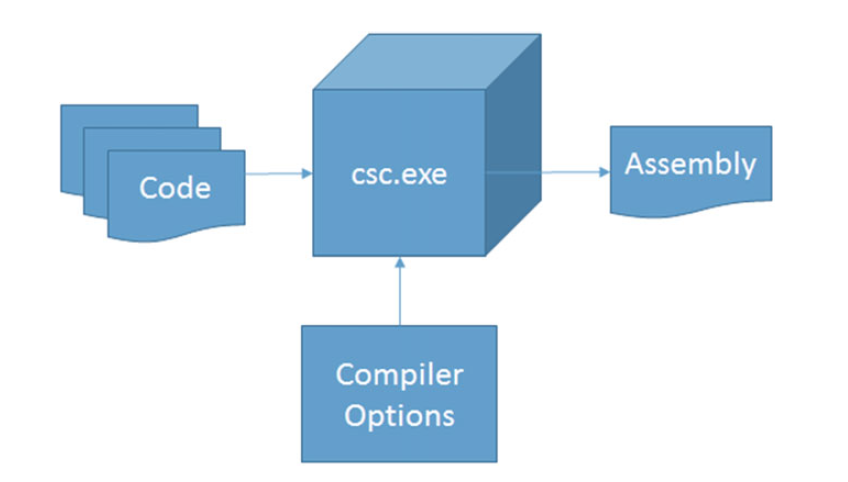
\includegraphics[scale=0.35]{img/compiler-as-a-black-box}
%		\caption{Compiler as a black box~\cite{dot-net-development-using-the-compiler-api}}
%		\label{fig:compiler-as-a-black-box}
%\end{figure}

Not only have been compilers for both Visual Basic and C\# rewritten into the entirely managed code\footnote{The term managed code refers to program source code written in one of high-level programming languages available for use with Microsoft .NET Framework, and require a Common Language Runtime virtual machine in order to be executed.}, they also expose the internals of the compiler pipeline via a public .NET API~\footnote{Application Programming Interface}. This makes them a platform (also known as \textit{compiler-as-as-service}) with rich code analysis APIs that can be leveraged by developers to perform analysis, code generation or dynamic compilation in their own programs~\cite{roslyn-succinctly}. Those can be then easily integrated into the Visual Studio all without the hard work of duplicating compilers' parsing logic.

This chapter will take a look at how the Roslyn API layers are structured, how the original source code is represented by the compiler and how developers can build tools upon the compiler's API. Note, that although Roslyn provides equivalent APIs for both VisualBasic and C\#, this thesis only focuses on the latter since it is relevant for the practical part of the thesis.  
  
\section{The Compiler Pipeline}
Roslyn compilers expose an API layer that mirrors the traditional compiler pipeline (see \ref{fig:roslyn-compiler-pipeline}). Instead of a single process of generating the target program, each compilation step is treated as a separate component~\cite{roslyn-overview}:

\begin{itemize}
  \item \textbf{Parse phase} consists of \textit{lexical analysis} (\textit{scanner}) and \textit{syntactic analysis} (\textit{parser}). First, the lexical analyzer processes the stream of characters from the source program and groups them into meaningful sequences called \textit{lexemes}. Those are subsequently processed by the \textit{syntax analyzer} that creates a tree-like structure of tokens based on the language grammar~\cite{dragon-book}.

  \item \textbf{Symbols and metadata phase} where named symbols are generated based on the declarations from the source and imported metadata.

  \item \textbf{Bind phase} in which the identifiers from the source code are matched to their respective symbols.

  \item \textbf{Emit phase} where all the gathered information is used to emmit an assembly.
\end{itemize}

\begin{figure}[h!]
		\centering
			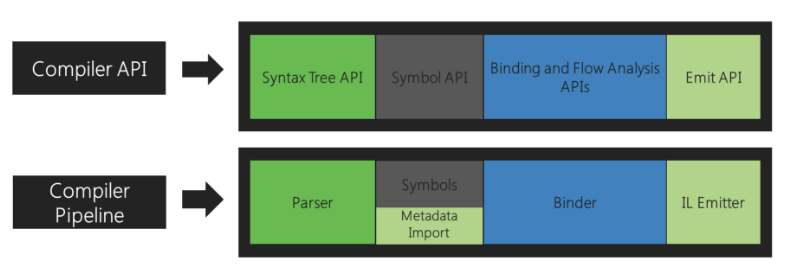
\includegraphics[scale=0.5]{img/roslyn-compiler-pipeline}
		\caption{Compiler pipeline~\cite{roslyn-overview}}
		\label{fig:roslyn-compiler-pipeline}
\end{figure}

In each phase, the .NET Compiler Platform creates an object model containing gathered information and exposes it through the API in form of .NET objects. These objects are also used internally by Visual Studio~\footnote{The new generation of Visual Stuio leveraging from the Roslyn compiler are called vNext and first one was VS 2015.} to support basic IDE functionality. For instance \textbf{syntax tree}, that is the result of the parse phase, is used to support formatting and colorizing the code in the editor. The result of the second phase -- \textbf{hierarchical symbol table}, is the basis for \textit{Object browser} and \textit{Navigate~to} functionality. Binding phase is represented as an \textbf{object model that exposes the result of the semantic analysis} and is utilized in \textit{Find all~references} or \textit{Go~to~definition}. Finally, the Emit phase produces the~Intermediate Language (IL) byte codes and is also used for \textit{Edit and~Continue} feature~\cite{roslyn-overview}.

\section{The .NET Compiler Platform's Architecture}
The Roslyn's architecture consists of two main layers - Compiler and Workspaces APIs, and one secondary layer - Features API, as seen on Figure~\ref{fig:roslyn-compiler-architecture}.

\begin{figure}[h!]
		\centering
			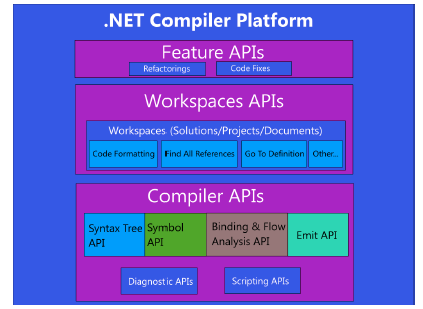
\includegraphics[scale=0.6]{img/roslyn-compiler-architecture}
		\caption{.NET Compiler Platform Architecture~\cite{roslyn-succincly}}
		\label{fig:roslyn-compiler-architecture}
\end{figure}

One of the key concepts of .NET Compiler Platform is immutability. The compiler exposes hundreds of types that represent all information about source code from \texttt{Project} and \texttt{Document} to \texttt{SyntaxTrees} with almost all of those types being immutable. This means, that once created, the object cannot change. In order to alter it in any way, new instance must be created, either manually, or from an existing instance by applying one of many \texttt{With()} methods that the API provides.

The immutability enables the compiler to perform parallel work without need to create duplicate objects or apply any locks on them. This concept is useful for the command line compiler but it is considered extremely important for IDEs where it enables for one document to be handled by multiple analyzers in parallel.

\subsection{The Compiler APIs}
As discussed in the previous section, the Compiler APIs offer an object model representing the results of syntactic and semantic analysis produced by the respective phases of the compiler pipeline. Moreover, it also includes an immutable snapshot of a single compiler invocation, along with assembly references, compiler options, and source files. This layer is agnostic of any Visual Studio components, and as such can be used in stand-alone applications as well. There are two separate, though very similar, APIs for Visual Basic and C\#, each providing functionality tailored for specific language nuances.

\subsubsection{Diagnostic APIs}
Apart from parsing code and producing an assembly, the compiler is also capable of raising diagnostics, covering everything from syntax to semantics, and report them as errors, warnings or information messages~\cite{roslyn-succinctly}. This is achieved through the compilers' Diagnostics APIs that allow developers to effectively plug-in to compiler pipeline, analyze the source code using the exposed object models, and surface custom diagnostics along with those defined by the compiler itself. These APIs are integrated to both MSBuild~\footnote{The Microsoft Build Engine https://github.com/Microsoft/msbuild} and Visual Studio (2015 and newer). providing seamless developer experience. The practical part of this thesis relies on Diagnostic APIs to provide custom diagnostics and the details will be discussed in Chapter \ref{chap:custom-roslyn-analyzers}.

\subsubsection{Scripting APIs}
As a part of the compiler layer, Microsoft team has introduced new Scripting APIs that can be used for executing code snippets. These APIs were not shipped with .NET Compiler Platform 1.0 and are part of v2.0.0 RC3\footnote{Release candidate 3, as per https://github.com/dotnet/roslyn/wiki/Scripting-API-Samples [26-02-2017].}.

\subsection{Workspaces APIs}
Workspace represents a collection of solutions, projects, and documents. It provides a single object model containing information about the projects in a solution and their respective documents; exposes all configuration options, assembly and inter-project dependencies, and provides access to syntax trees and semantic models. It is a starting point for performing code analysis and refactorings over entire solutions.

Although it is possible to use the \texttt{Workspace} outside of any host environment, the most common use case is an IDE providing an instance of \texttt{Workspace} that corresponds to the open solution. Since the instances of \texttt{Solution} are immutable, the host environment must react to every event (such as user key stroke) with an update of the \texttt{CurrentSolution} property of the \texttt{Workspace}.

\subsection{Feature APIs}
This layer relies on both compiler and workspaces layers and is designed to provide API for offering code fixes and refactorings. Features APIs were also utilized while working on the practical part of this thesis.
  
\section{Syntax Tree}
As mentioned in the previous sections, the product of the syntactic analysis is a syntax tree. It enables developers to work with the code in a managed way instead of working against plain text. Syntax trees are used for both analysis and refactorings, where the new code is generated either manually or as a modified version of the existing tree. While being immutable, syntax trees are thread-safe and analysis can be done in parallel.

It is important to point out, that in a same way the compiler constructs a syntax tree from the source text, it is also possible to round-trip back to the text representation. Thus, the source information is always preserved in full fidelity. This means that every piece of information from source must be stored somewhere within the tree, including comments, whitespaces or end-of-line characters, which is a major difference to the general concept of compilers discussed in Chapter~\ref{chap:compilers}

Figure~\ref{fig:roslyn-syntax-tree} shows a syntax tree of an invocation expression as obtained from Syntax Visualizer\footnote{https://roslyn.codeplex.com/wikipage?title=Syntax\%20Visualizer} extension available in Visual Studio. This tool is useful for understanding how Roslyn represents particular language constructs and is widely utilized whenever one needs to analyze the code. Following sections explain what are the main building blocks of such syntax tree, referring to Figure~\ref{fig:roslyn-syntax-tree}

\begin{figure}[h!]
		\centering
			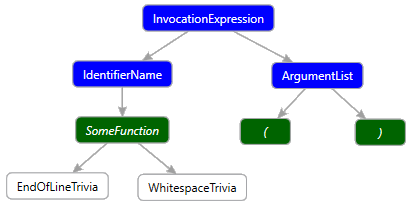
\includegraphics[scale=0.8]{img/roslyn-syntax-tree-2}
		\caption{Syntax tree of an invocation expression}
		\label{fig:roslyn-syntax-tree}
\end{figure}

\subsubsection{Syntax Nodes}
Syntax nodes (blue color) are non-terminal nodes of a syntax tree, meaning they always have at least one other node or token as a child. Nodes represent syntactic constructs of a language such as statements, clauses or declarations. Each type of node is represented by a single class deriving from \texttt{SyntaxNode}. Apart from common properties \texttt{Parent}, \texttt{ChildNodes} and utility methods like \texttt{DescendantNodes}, \texttt{DescendantTokens}, or \texttt{DescendantTrivia}, each subclass exposes specific methods and properties. As shown in Figure~\ref{fig:roslyn-syntax-tree}, \texttt{InvocationExpression} has two properties, \texttt{IdentifierName} and \texttt{ArgumentList} both of which are \texttt{SyntaxNodes} themselves.
 
\subsubsection{Syntax Tokens}
As opposed to nodes, syntax token (green color) represent terminals of the language grammar, such as keywords, punctuation, literals and identifiers. For the sake of efficiency, \texttt{SyntaxToken} is implemented as a value type (C\# structure) and there is only one for all kinds of tokens. To be able to tell them apart, tokens have \texttt{Kind} property. For example, \texttt{SomeFunction} is of kind \texttt{IdentifierName}, whereas "\texttt{(}" character is \texttt{OpenParenToken}.

\subsubsection{Syntax Trivia}
In order to enable refactoring features, syntax trees must also store information about whitespaces, comments and preprocessor directives that are insignificant for compilation process itself. This information is represented by another value type -- \texttt{SyntaxTrivia} (white color). Trivia are not really parts of the tree itself, rather they are properties of tokens accessible by their \texttt{LeadingTrivia} and \texttt{TrailingTrivia} collections.

\section{Semantics of the Program}
As explained in Chapter~\ref{chap:compilers}, even though syntax trees are enough to describe the proper form of the program (compliance to the language grammar), they cannot enforce all language rules, for example, type checking. In order to tell whether a method is called with the right number of arguments, or operator is applied to operands of the right type, it's inevitable to introduce semantics. 

Its one of the core compiler's responsibilities to populate symbol tables with information about all elements and their properties from the source program. Attributes such as identifier name, type, allocated storage, scope; or for method names the number and types of arguments and their return values; are all stored in order to be utilized later when producing intermediate language.

\subsubsection{Symbols}
In .NET Compiler Platform, a single entry of a symbol table is represented by a class deriving from \texttt{ISymbol}. The symbol represents every distinct element (namespace, type, field, property, event, method or parameter) either declared in the source code or imported as metadata from a referenced assembly. Each specific symbol has its own methods and properties often directly referring to other symbols. For example \texttt{IMethodSymbol} has a \texttt{ReturnType} property specifying what is the type symbol the method returns.

\subsubsection{Compilation}
An important immutable type, that represents everything needed to compile a C\# (or Visual Basic) program is a \texttt{Compilation}. It contains all source files, compiler options and assembly references. Compilation provides convenient ways to access any discovered symbol. For instance, it is possible to access the entire hierarchical symbol table rooted by global namespace, or look up type symbols by their common metadata names.

\subsubsection{Semantic Model}
When analyzing a single source file of a compilation, all its semantic information is available through a \textit{semantic model}. The \texttt{SmeanticModel} object can answer many questions such as:
  \begin{itemize}
  \item What symbol is declared at the specific location in the source?
  \item What is the result type of an expression?
  \item What symbols are visible from this location?
  \item What diagnostics are reported in the document?
  \end{itemize}
 
This makes semantic model very useful when performing static code analysis concerned with more than just syntax.
 
\pagebreak
\section{Analysers and Code Refactorings}
[3 pages?]
  
%  - how to perform static code analysis with Roslyn
%    - writing anlyzers and code fixes / code refactorings  

% =================================================================
% ============================= CHAPTER 5 =========================
% =================================================================
\chapter{Implementation of Custom Analyzers}
\label{chap:custom-roslyn-analyzers}
\section{Kentico CMS Internal Guidelines}

What is Kentico CMS?
how big the solution is, how old, extremely much knowledge accumulated in 12 years. some technologies were developed even before Microsft had them in .NET
Many helpers etc. code style and onther conventions
need to be followed during development and chceked in code reviews

What was implemented is not really an "automated code review" - only specific ruleset will be implemented in Roslyn and rules will be applied live while writing code in VS. -- it does not really replace manual code review, only takes the burden off reviewer to check for most common mistakes.
\subsection{The Specificities of Kentico CMS Solution}
Measurements from roslyn - number of projects, documents, nodes... show table, reference to code that produces it (shall be included in IS)

not only is onboarding of new employees complicated but the code review process is really hard, reviewer needs to think about many things and impacts the changes might have
it's very easy that some bugs or uncomplient code will slip under his nose
more and more helpers created and not everything is shared on skype/ you might miss something

this led to need for some automated way to check the compliance with internal guidelines

\subsection{Old BH}
Tools for static code analysis in general

one such tool was BH
company did not have the motivation to invest too much into creating extremely complicated tool and at the time (YYYY) it was very difficult to create something custom which would be robust and almost perfect at the same time

-  first attempts to rewrite BH to Roslyn 
not so successful Bachelor thesis by another student (huge performance problems, implementation basically one to one with the old console app, does not leverage of Roslyn type system, everything based on strings, therefore many missed diagnostic problems)

Does run on CI

Problems to be addressed

\subsubsection{More robust model building}
no dependance on code style, 
fully qulified names, 
alias imports that could ruin the following analysis
string checks. if additional space is there, most checks will just ignore

\subsubsection{Need for semantic categories}
many cases that were not discoverable by string comparison were uncovered

where old tool searched for HttpRequest.Cookies - if someone saved the request into variale no way for  old bh to diagnose the usage.. with roslyn and semantic analysis it is an easy task
    
\subsubsection{Ease of use}
integrated in IDE, run in paralled with programmer typing... almost no one run BH before making push.. like this with no warning  policy they cannot do it

old BH reporting not integrated in VS -> almost no one runs it locally, they need to wait for CI to tell them what went wrong



\subsubsection{Configuration}
talk about the old configuration of the BH, and how this one maps to Roslyn version (suppression pragmas vs supression files, some analyzers look at the filepath or file extension directly.. some chcecks like SystemIO had to be supressed - level set to none in ruleset file - for files that it did not make sense for... helpers that wrap the "forbidden" functionality were marked with pragma statements around the whole class so that it is clearly visible in code)

cumbersome configuration - cannot ignore one usage, therefore all files/folders/projects were ignored for some checks


\subsection{Roslyn attempts}
tell about how resharper, fxcop and stylecop are (not)used
talk very briefly about the intentions to rewrite bh to roslyn - bachelor thesis, not so successful, only syntax and very early stage of Roslyn itself.. too many exceptions thrown when using the tool, and therefore extremely slow performance which made it practically unusable

\subsection{Limitations}
not only C\# but also some project specific stuff in XMLs and few JS checks like no xdescribe/xit

some checks were not needed anymore and were just obsolete or even turned off

why we are only concerned with this and do not check the naming conventions or advanced refactoings - tools already exist for this (StyleCop and ReSharper) and were not implemented in new BH version - usings sorting and such is provided by other tools

....
wuhuuu and here comes our part..

\section{Requirements and Categorization}
There is differend concern about categorizing the domain specific stuff about the implemented analyzers and then the C\# and compiler specific things that are used when implementing it.. therefore helpers for SMAE, CAE, IE... explain... new language version - new approach but same domain is concerned '.' vs '?.'


compare to old BH, where this was more project and file based
define two nugets - whi Web.Analyzers - specificities for CMSApp project
other semantic categories, what they represent


\section{Architecture}
Main concern are ApiReplacement and General (string) and Internal ApiGuidelines --> need for analyzing members of certain types

\subsection{CMSApiReplacement}
Example + why

\subsubsection{For Member}
define strategies for SimpleMemberAccessExpression and ConditionalAccessExpression analysis grouped by strategy for ApiReplacementForMemberAnalyzer - this one is used as strategy in all relevant analyzers and is configured via ApiReplacementConfig class defining Rule, ForbiddenMembers and ForbiddenTypes.... use examples... tell how it is important not to access semantic model straight away and do basic analysis on syntax first
how strategies are extendable, when new language feature is presented
how they are configurable to use any DIagnosticFormatter desired

UML

\subsection{For Method}
more involved analysis.. MemberInvocationAnalyzer used by ApiReplacementForMethodAnalyzer... callback on SyntaxKind.InvocationExpression

UML 
it is easy to access semantic model first and analyze the IMethodSymbol... however.. point out how many times this callback is invoked and how many times SemanticModel would have been queried... therefore very simple semantic for getting rid of cases that do not have to be analyzed further... tell about the possible cases of InvocationExpression - nested SimpleMemberAccess.. first MemberBindingExpression, or IdentifierName... always show a graph...
if it could be skipped based on syntax - invoked method name is for sure none of the forbidden member names, skip, otherwise, analyze further based on semantics

TEMPLATE METHOD - used not only for straightworward API replacements but also for conformance toAPI usage guidelines - therefore need to be configurable - explain that the logis of 'forbidden member and type' is the same

!!!!do some benchmarking how this heuristic helped with the performance!!!! show graph

\subsubsection{CmsApiGuidelines}
use mostly MethodInvocationAnalyzer and leverage its template method pattern, to dig deeper into analysing where the method was invoked or who it is invoked - which overload is called, is it using predefined constants instead of plain string etc... (limitations)

\subsubsection{AbstractionOverImplementation}
Why lucene - 3rd party libs and assembly binding, bound to IdentifierName  - tell how many, therefore it is crutial to make it fast and cout of as soon as possible

\subsubsection{StringMethodsAndCulture}
Why,
How - do not use MethodInvocationAnalyzer - some performance gain as we do not need to configure the forbidden types from the outside, we know string is always the ReceiverType and it is a sealed class and thus no need to analyze its parents, interfaces etc.
Invocation is analyzed if it supplied the correct arguments... StringComparison or CultureInfo

Methods ToLower and ToUpper have specific overloads in Kentico that accept CultureInfo because of problems with specific turkish culture (TODO search for some reference on wiki)

\subsection{CodeFixes}
Why
How - CMSApiReplacements - pretty straightforward, although some limitations in conditional accesses that do not have the codefix ... analyze why this is hard, can talk about the tree structure
SystemIO does not have a codefix as this would be extremely tough to implement not a clear 1 to 1
Lucene easy, then things like not using the DB layer from Presentation is not clear how to fix and it is needed for developer to chande the design of the solution to avoid this
API guidelines have mostly easy fixes - suggesting different usages/overloads/methods

\subsection{Tests}
concerns about strings everywhere - attempts to use nuget with kentico libraries - many problems - could not be portable, nuget size was enormous - some wierd feeling of recurrsion... no other libraries seem to have been experiencing similair issues..

so libs are only referenced in tests - explain why this is important (when creating a compilation - metadata references need to be added)
measures taken to eliminate any typos - could not pass the test if the source code itself is not compilable - this is for example how the ever present bug in original BH was discovered Response vs Request.Redirect() !!! would not be possible without nuget and additional effor to make all tests compilable

tests not only for BH but of course for all other helpers/utils/extensions

(- how to actually know we are looking for right things and did not misspell something --> tests always reference current version of Kentico.Libraries (NuGet package). If there is any typo in either source code of test files or analyzers, the tests will fail (needed to manually turn this feature on since the boilerplate generated by Microsoft project did not support this))

\subsection{Roslyn as SDK and Its Usage -- Considerations and Remarks}
Changing versions ... not really well documented
Only issues on GH provide some insight
e.g. SkipGeneratedCoOdeAnalysis or RunAnalyzersInParallel - some discussions on GitHub but not clear outcomes, sometimes proposition does not math the actual implementation and it is generally hard to find some best practices on how to do stuff ad it is still a pretty young tech... moreover the examples are not really updated according to new versions of the API so one struggles with implemeting something on his own only to find a few weeks later that it was added or it is considered for the next milestone

many useful things are marked as internal in the source code and there are many issues on GH to make them public

current version used is v.1.3.X and for this on VS with Update 3 is needed... had to be installed on all build boxes to accomodete BH depoloyment

... version v2 was released after the implemetnation was finished and it was considered although it was agreed we will not use it as it required VS2017 and nobody is happy about it.. talk about some cons...

(  - ConfigureGeneratedCodeAnalysis - big boost when roslyn API allowed to opt out for analyzer to be run on generated code. Before, heuristics had to be performed by analyzers themselves on every callback
   https://github.com/dotnet/roslyn/issues/6998
   https://github.com/dotnet/roslyn/pull/7526)

\subsection{Concerns about performance}
somehow explain why... and introduce following chapter

% =================================================================
% ============================= CHAPTER 6 =========================
% =================================================================
\chapter{Measuring and Optimizing the Performance}
Why tool needs to be super-fast (refer to chapter 4 where this should have been said)

Talk about /ReportAnalyzer switch of MSBuild process (csc.exe)

How the performance of the slowest analyzers (SystemIO, BaseChecks) was improved

Talk about how analyzers deployment influenced the build time

Questionares sent to development team, feedback from senior developers

% =================================================================
% ============================= CHAPTER 7 =========================
% =================================================================
\chapter{Conclusion}
  - what issue it solved
  - what is the current status of the project
  - how it helped the development teams...
  - how to maintain the tool, 
  - how easy it is to add new analyzers, 


% =================================================================
% =============================== STUFF ===========================
% =================================================================
	% From template
	\makeatletter\thesis@blocks@clear\makeatother
	\phantomsection %% Print the index and insert it into the
	\addcontentsline{toc}{chapter}{\indexname} %% table of contents.

	\printindex
    
% =================================================================
% =========================== BIBLIOGRAPHY ========================
% =================================================================
  \printbibliography

% =================================================================
% ============================ APPENDICES =========================
% =================================================================    
	\appendix %% Start the appendices.
  \chapter{Source Codes in IS}
  \chapter{Questionnaires}
TODO...

  \chapter{Deployment and Versioning}
[2 pages]

\end{document}
